\begin{center}
  \textsf{Листок 3.}
\end{center}
\vspace{0.01mm}
\hrule

\taskpic{Край гладкого горизонтального стола скруглён по окружности
  радиуса $R$. С какой наименьшей скоростью надо пустить тело, чтобы
  оно, достигнув скругления, сразу полетело по
  пораболе?. }{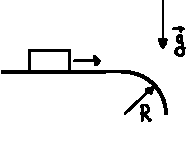
\includegraphics[width=4cm]{p09_9.pdf}}

\taskpic{По деревянным сходням, образующим угол $\alpha$ с горизонтом,
  втаскивают за привязанную к нему верёвку ящик. Коэффициент трения
  ящика о сходни $k$. Под каким углом к горизонту надо тянуть верёвку,
  чтобы с наименьшим усилием втащить ящик? }{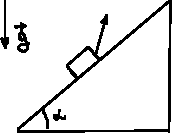
\includegraphics[width=4cm]{p09_10.pdf}}

\taskpic{Тело массы $m_1$ лежит на доске массы $m_2$, находящейся на гладкой
  горизонтальной поверхности. Коэффициент трения между телом и доской
  $k$. Какую силу надо приложить к доске, чтобы тело соскользнуло с
  неё. За какое время тело соскользнёт, если к доске приложена сила
  $F_0$, а длина доски $l$.  }{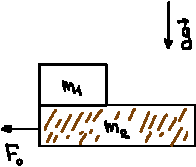
\includegraphics[width=4cm]{p09_11.pdf}}

\taskpic{Между двумя одинаковыми гладкими брусками массами $m_1$ каждый
  вставлен клин массы $m_2$ с углом $\alpha$. Определите ускорение
  тел. }{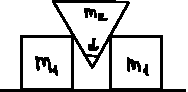
\includegraphics[width=4cm]{p09_12.pdf}}
